\documentclass[12pt]{article}
\usepackage[top=1cm, bottom=3cm, right=2cm, left=2cm]{geometry}
\usepackage{amsfonts, amssymb, amsmath, hyperref}
\usepackage{graphicx}
\usepackage[T1, T2A]{fontenc} % T2A for Cyrillic font encoding
\usepackage[english, russian]{babel}
\usepackage[justification=centering]{caption}
\usepackage{wrapfig,lipsum,booktabs}
\usepackage{placeins}
\usepackage{subcaption}
\usepackage{multirow}
\usepackage{indentfirst}
\usepackage{bm}
% \usepackage{lmodern} % Add this line to use the Latin Modern font

\begin{document}
\title{\textbf{Лабораторная работа 4.1.1}\\ [2pt]{Геометрическая оптика}}
\date{\today}
\author{Татаурова Юлия Романовна}

\begin{document}
\maketitle
\section*{Аннотация}
В работе были вычислены фокусные расстояния линз разными способами. Был cобран телескоп Кеплера и проекционный микроскоп.
\section*{Цель работы}
Изучить методы определения фокусных расстояний линз и сложных оптических систем;изучить модели зрительных труб (астрономической трубы Кеплера) и микроскопа, определить их увеличения.

\section*{Теоретические сведения}
\subsection*{Определение фокусного расстояния собирающих линз и сложных оптических систем по методу Бесселя}

Схема метода Бесселя для случая, когда $n = n'$ и $f' = -f$, представлена на \ref{fig:bessel}. Она основана на том, что при заданном расстоянии $L$ между предметом и экраном уравнение (1.24) представляет собой квадратное уравнение относительно расстояния $s$ от главной плоскости пространства предметов до предмета ($s < 0$):

\begin{equation}
\frac{1}{s} + \frac{1}{L - \delta + s} = \frac{1}{f},
\label{eq:bessel}
\end{equation}

имеющее при условии $L > 4f + \delta$ решения $s_1$ и $s_2$, показанные на рис. 2, где $\delta$ — расстояние между главными плоскостями системы (линзы).

\begin{figure}[h]
\centering
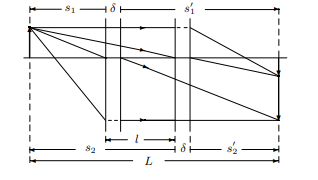
\includegraphics[width=0.7\textwidth]{images/bessel_method.png}
\caption{Измерение фокусного расстояния оптической системы по методу Бесселя}
\label{fig:bessel}
\end{figure}

С учётом симметрии и направлений измерения расстояний, положения предметов определяются соотношениями $s_2' = -s_1$ и $s_1' = -s_2$. Для расстояния $L$ между предметом и экраном и расстояния $\ell$ между двумя положениями системы (линзы) получаем: $L - \delta = s_1' - s_1$,

\begin{equation}
\ell = -s_2 + s_1 = s_1 + s_1'.
\label{eq:ell}
\end{equation}

Отсюда следует, что

\begin{equation}
s_1 = -\frac{1}{2}(L - \delta - \ell), \quad s_1' = \frac{1}{2}(L - \delta + \ell).
\label{eq:positions}
\end{equation}

Подставляя (\ref{eq:positions}) в формулу (1.22), после преобразований находим выражение:

\begin{equation}
f = \frac{(L - \delta)^2 - \ell^2}{4(L - \delta)}.
\label{eq:f_delta}
\end{equation}

Если выполняется условие $|\delta| \ll L$, то с относительной погрешностью

\begin{equation}
\varepsilon_f = \frac{L^2 + \ell^2}{L^2 - \ell^2}
\label{eq:error}
\end{equation}

формула (\ref{eq:f_delta}) может быть представлена в более простом виде:

\begin{equation}
f = \frac{L^2 - \ell^2}{4L}.
\label{eq:f_simple}
\end{equation}

Для определения фокусного расстояния $f$ достаточно измерить расстояние $L$ между предметом и экраном и расстояние $\ell$ между двумя положениями системы, при которых на экране видны чёткие изображения. 

Если выполнить измерения для двух пар величин $L$ и $\ell$, то из двух уравнений вида (\ref{eq:f_delta}) можно найти обе характеристики системы: $f$ и $\delta$.

При выводе формул (\ref{eq:bessel})–(\ref{eq:error}) предполагалось, что расстояние между главными плоскостями системы положительно ($\delta > 0$), однако полученные результаты справедливы и для $\delta \leq 0$.

\subsection*{Определение фокусного расстояния тонкой собирающей линзы и сложных оптических систем по методу Аббе}

Измерение фокусного расстояния по методу Аббе основано на определении поперечного увеличения для нескольких (не менее двух) различных положений предмета, находящегося на оптической оси исследуемой оптической системы.

\begin{figure}[h]
\centering
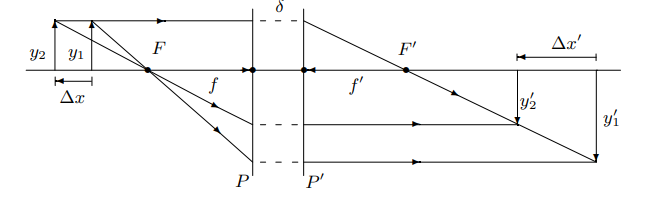
\includegraphics[width=0.7\textwidth]{images/abbe_method.png}
\caption{Измерение фокусного расстояния оптической системы по методу Аббе}
\label{fig:abbe}
\end{figure}

Фокусное расстояние системы можно выразить через положения предмета и соответствующие увеличения следующим образом:

\begin{equation}
f = \frac{\Delta x}{\Delta (y/y')} = -\frac{\Delta x'}{\Delta (y'/y)},
\label{eq:abbe}
\end{equation}

где:
$\Delta x = x_2 - x_1$ — смещение предмета,
$\Delta x' = x_2' - x_1'$ — соответствующее ему перемещение изображения,
$\Delta (y'/y) = y_2 / y_2' - y_1 / y_1'$ — приращение поперечного увеличения,
$\Delta (y/y')$ — приращение величины, обратной поперечному увеличению.

Для повышения точности измерений следует выбирать такие смещения $\Delta x$, чтобы увеличения заметно отличались друг от друга. С целью уменьшения случайной ошибки, возникающей при фокусировке изображения, измерения следует проводить несколько раз, усредняя полученные данные.

Основное достоинство метода Аббе состоит в том, что фокусное расстояние сложной системы или линзы, как это видно из рисунка, может быть получено при неизвестном расстоянии $\delta$ между главными плоскостями $P$ и $P'$.
\subsection*{Микроскоп}

Микроскоп состоит из двух собирающих систем линз — объектива и окуляра, расположенных на расстоянии $t_{12}$ друг от друга в трубе, называемой тубусом. Длина тубуса у всех микроскопов, выпускаемых отечественной промышленностью, составляет 16 см, что значительно превышает фокусные расстояния объектива и окуляра. Предмет помещается на малом расстоянии перед передним фокусом объектива. Между предметом и объективом может находиться иммерсионная жидкость с показателем преломления $n$, тогда такой микроскоп называется \textit{иммерсионным}.

\begin{figure}[h]
\centering
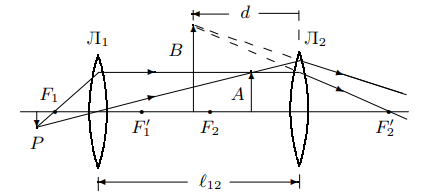
\includegraphics[width=0.7\textwidth]{images/microscope_scheme.png}
\caption{Ход лучей в микроскопе}
\label{fig:microscope}
\end{figure}

Объектив $J_1$ даёт действительное перевёрнутое увеличенное изображение $A$ предмета $P$, которое рассматривается через окуляр $J_2$, действующий как лупа. Мнимое изображение $B$, даваемое окуляром, располагается на некотором расстоянии $d$ от окуляра. Наводя микроскоп на резкость, наблюдатель автоматически устанавливает такое расстояние $d$, которое удобно для аккомодации глаза.

Фокусные расстояния микроскопа как сложной системы даются формулами:

\begin{equation}
f_M = -\frac{f_1 f_2}{\Delta}, \quad f_M' = \frac{f_1' f_2'}{\Delta},
\label{eq:microscope_focal}
\end{equation}

где $\Delta$ — оптический интервал. Для безиммерсионного микроскопа ($n = n' = 1$), для которого $f_1 = -f_1' > 0$, $f_2 = -f_2' > 0$, увеличение выражается как:

\begin{equation}
N_M = \frac{L}{f_M} = -\frac{\Delta L}{f_1 f_2}, \quad \Delta = t_{12} - f_1 - f_2.
\label{eq:microscope_magnification}
\end{equation}

Величину $N_M$ можно представить в виде произведения увеличений объектива и окуляра:

\begin{equation}
N_M = N_1 N_2, \quad N_1 = -\frac{\Delta}{f_1}, \quad N_2 = \frac{L}{f_2}.
\label{eq:components}
\end{equation}

Для иммерсионного микроскопа увеличение (\ref{eq:microscope_magnification}) надо умножить на $n$ — показатель преломления иммерсионной жидкости.

\subsection*{Зрительные трубы}

Зрительные трубы, основными элементами которых являются объектив и окуляр, предназначены для наблюдения удалённых предметов. Уменьшенное обратное изображение $A$ удалённого предмета, даваемое объективом, находится практически в его фокальной плоскости. Мнимое изображение $B$, даваемое окуляром, располагается на расстоянии $d$ от окуляра.

\begin{figure}[h]
\centering
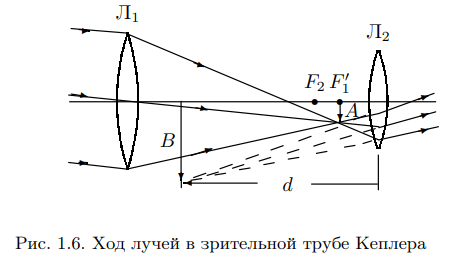
\includegraphics[width=0.7\textwidth]{images/telescope_scheme.png}
\caption{Ход лучей в зрительной трубе Кеплера}
\label{fig:telescope}
\end{figure}

В теории зрительных труб считается, что глаз аккомодирован на бесконечность. При этом мнимое изображение $B$ должно располагаться в бесконечности, и, следовательно, промежуточное изображение $A$ должно находиться в фокальной плоскости окуляра, а задний фокус объектива должен быть совмещён с передним фокусом окуляра. В таком случае зрительные трубы представляют собой телескопические системы.

\section*{Экспериментальная установка}
\textbf{Оборудование:}оптическая скамья, набор линз, экран, осветитель со шкалой, зрительная труба, диафрагма, линейка.\\

\indent Все элементы оптической системы должны быть центрированы относительно оптической оси: выставлены по высоте и по поперечному положению. Поэтому перед началом работы отцентрируем систему. Порядок центровки следующий:\\

\noindent\textbf{1)} Установили источник в начале оптической скамьи и направили его вдоль скамьи.\\
\textbf{2)} Установили подзорную трубу вдоль скамьи так, чтобы её объектив оказался непосредственно напротив источника; выровняли их по высоте и по поперечному расположению.\\
\textbf{3)} Установили экран непосредственно перед источником и выровняли его по высоте и поперечному смещению так, чтобы центр светового пятна от источника совпадал с центром экрана.\\
\textbf{4)} Для центровки первой собирающей линзы поставили её между уже центрированными источником и экраном. Убедились, что плоскость линзы была перпендикулярна оптической скамье. Отрегулировали положение линзы по высоте и в боковом направлении так, чтобы центр светового пятна снова оказался в центре экрана. Перемещая линзу вдоль скамьи, уточнили её центровку. Зафиксировали крепёжные винты линзы.\\
\textbf{5)} Добавляли следующие линзы последовательно, устанавливая их между предыдущей линзой и экраном. Центрировали положение пятна на экране, изменяя положение только добавляемой линзы.\\

\subsection*{I. Определение фокусных расстояний линз с помощью подзорной трубы}

\indent \textbf{1)}Настроили подзорную трубу так, чтобы она была сфокусирована на «бесконечность». Наведя трубу на далёкий предмет и с помощью фокусировочного винта трубы получили чёткое изображение предмета.\\

\indent \textbf{2)}Расположили одну из линз на оптической скамье перед источником света на расстоянии, приблизительно равном фокусному. Далее за линзой разместили подзорную трубу \\

\begin{figure}[h!]
    \centering
    \begin{subfigure}{0.45\linewidth}
        \centering
        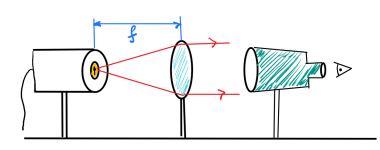
\includegraphics[width=8cm]{images/setup1.png}
        \caption{Схема установки для измерения фокусных расстояний собирающих линз}
    \end{subfigure}
    \hfill
    \begin{subfigure}{0.45\linewidth}
        \centering
        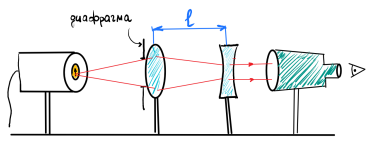
\includegraphics[width=8cm]{images/setup1(2).png}
        \caption{Схема установки для измерения фокусного расстояния рассеивающей линзы}
    \end{subfigure}
\end{figure}

\indent \textbf{3)}Далее разворачивали линзы и измеряли их фокусные расстояния. Результат измерений приведен ниже.

\begin{table}[h]
    \centering
    \begin{tabular}{|c|c|c|}
        \hline
        № линзы & $F_1$, см   & $F_2$, см   \\ \hline
        4.6     & 4.2       & 4.8       \\ \hline
        4.2     & 10.1      & 10.2      \\ \hline
        4.1     & 4.1       & 4.9       \\ \hline
        4.4     & 18.3      & 17.5      \\ \hline
        4.3     & 12.2      & 12.4      \\ \hline
    \end{tabular}
    \caption{Результы измерений фокусных расстояний с помощью подзорной трубы}
\end{table}

\indent Повторяя измерения нескоько раз для одной линзы, каждый раз заоново выставляя линзу, мы получали одинаковые результаты, поэтому среднеквадратичное отклонение далее не будем учитывать. Поэтому погрешность измерения фокусного расстояния $\bm{\sigma_F = 0.1}$ \textbf{см}.

\indent \textbf{Вычислили фокусное расстояния рассеивающей линзы}.\\
\textbf{а)} Разместили на скамье перед источником вспомогательную положительную линзу (линза №4.2 с фокусом $F$ $\approx$ 10 см) и получили на экране за линзой чёткое изображение предмета. Измерили расстояние от линзы до экрана $\bm{a_0 = 20\pm0.1 }$ \textbf{см}. \\
\textbf{b)} Использовали полученное изображение в качестве мнимого предмета для рассеивающей линзы: поместили отрицательную линзу между положительной и экраном. \\
\textbf{c)} Убрали экран и за отрицательной линзой разместили подзорную трубу. Перемещая отрицательную линзу по скамье (положительная оставалась неподвижной), получили сфокусированное изображение предмета в подзорную трубу. \\
\textbf{d)} Измерили расстояние $\bm{l = 17.9 \pm 0.01 }$\textbf{ см} между положительной и отрицательной линзами. Определили фокусное расстояние отрицательной линзы. \\
\begin{equation}
    \bm{F_{\text{отр}} = a_0 - l = -2.1 \pm 0.02} \textbf{ см}
\end{equation}

\subsection*{II. Измерение фокусных расстояний линз по формуле тонкой линзы и
методом Бесселя}
Использовалась линза №4.2 c фокусным расстоянием $F \approx 10$ {см}.
Поместив исследуемую линзу между источником и экраном и найшли два её
положения, при которых на экране возникают чёткие действительные изображения
— в одном случае увеличенное, а в другом уменьшенное. Соответственно $\bm{s_1 = 21\pm0.1}$ \textbf{см} и $\bm{s_2 = 28.7 \pm 0.1}$ \textbf{см}. Смещение между этими положениями $\bm{l = s_2 - s_1 = 7.7 \pm 0.2}$ \textbf{см}. Расстояние от источника до экрана $\bm{L = 51.2 \pm 0.1}$ \textbf{см}.
\begin{figure}[h!]
    \centering
    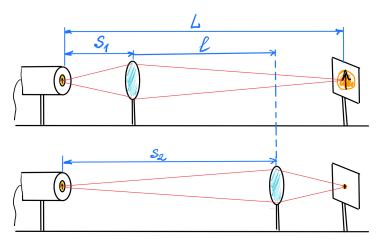
\includegraphics[width=8cm]{images/setup2.png}
    \caption{Схема установки для измерения фокусных расстояний собирающих линз по формуле тонкой линзы}
\end{figure}
Тогда по формуле тонкой линзы:
\begin{equation}
    \frac{1}{F} = \frac{1}{s} + \frac{1}{L - s}
\end{equation}

$$\bm{F_1 = 12.6\pm 0.2 \textbf{см}; F_2 = 12.4\pm0.2 \textbf{ см}}$$

По приближенной формуле Бесселя:
\begin{equation}
    \bm{F = \frac{L^2 - l^2}{4L} = 12.5 \pm 0.03} \textbf{ см}
\end{equation}

Далее повернув лину другой стороной повторили измерения:
$$\bm{s_1 = 21 \pm 0.1 \textbf{ см}; s_2 = 28 \pm 0.1 \textbf{ см}} $$
Тогда по формуле тонкой линзы:
$$\bm{F_1 = 12.6 \pm 0.2 \textbf{ см}; F_2 = 12.4 \pm 0.2 \textbf{ см}} $$
По приближенной формуле Бесселя:
$$\bm{F = 12.5 \pm 0.03 \textbf{ см}}$$

\subsection*{III. Измерение фокусных расстояний методом Аббе}
\textbf{1)} Установили линзу между осветителем с транспарантом - предметом известного размера $\bm{y_0}$ - и экраном. Получили на экране сфокусированное действительное изображение предмета и измерили его линейный размер $\bm{y_1}$.\\ 

\textbf{2)} Отодвинули осветитель на некоторое расстояние ${\Delta x}$ от линзы (линза оставалась неподвижной), измерив величину смещения. Затем придвинули экран к линзе на расстояние ${\Delta x'}$ до получения сфокусированного изображения. Измерили новый размер изображения ${y_2}$. \\

\textbf{3)} Рассчитали фокусное расстояние линзы методом Аббе:
\begin{equation}
    f = \frac{\Delta x'}{y_1 / y_0 - y_2 / y_0} = \frac{\Delta x}{y_0 / y_2 - y_0 / y_1}
\end{equation}

\begin{table}[h!]
    \centering
    \begin{tabular}{|c|c|c|c|c|c|c|c|}
        \hline
        Cторона линзы & $y_0$, см & $y_1$, см & $y_2$, см & $\Delta x$, см & $\Delta x'$, см & $f$, см & $f'$, см \\\hline
        Прямая   & 2 & 3 & 2   & 3 & 4.6 & 9.2 $\pm 1.1$ & 9.1 $\pm$ 1.05\\\hline
        Обратная & 2 & 2 & 1.5 & 3 & 2.3 & 9.2 $\pm 1.15$ & 9.1$\pm 1.1$ \\\hline
    \end{tabular}
    \caption{Данные для определения фокусного расстояния методом Аббe\\($\sigma_y = 0.05$ см; $\sigma_{\Delta{x}} = 0.1$ см)}
\end{table}



\begin{figure}[h!]
    \centering
    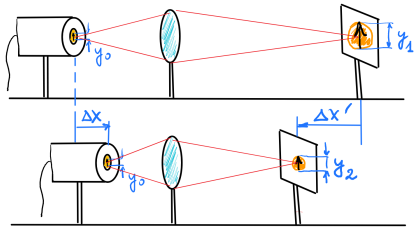
\includegraphics[width=8cm]{images/setup3.png}
    \caption{Схема установки для измерения фокусных расстояний собирающих линз методом Аббе}
\end{figure}

\subsection*{IV. Сборка и изучение подзорных труб Кеплера и Галилея}
\textbf{1)} Из имеющегося набора линз выбрали три: две линзы для объектива и окуляра (№4.3 $F_3 = 12.2 $см и №4.6 $F_6 = 4.8 $см), а также одну из собирающих линз для использования в качестве коллиматора(№4.4 $F_4 = 18.3 $см).\\

\textbf{2)}\textit{Настройка коллиматора}: \\
С помощью подзорной трубы установили коллиматорную линзу перед источником так, чтобы транспарант оказался строго в фокусе линзы. Таким образом создали расположенный на бесконечности предмет, который затем рассматривали с помощью модели телескопа. \\

\textbf{3)}\textit{Измерение углового размера}: \\
Глядя в окуляр вспомогательной подзорной трубы, оценили, сколько ячеек сетки изображения укладывается в круг радиуса риски. Так же посчитали и для увеличенного изображения. $a_1^2 \cdot n_1 = a_2^2 \cdot n_2$, где $a_1, a_2$ - размеры ячеек, $n_1, n_2$ - количество, укладывающихся квадратов. Отсюда получаем $\bm{\gamma_{\text{экс}} = \frac{a_2}{a_1} = \sqrt{\frac{n_1}{n_2}} = \sqrt{\frac{11}{5}} = 1.5\pm0.8}$ Здесь погрешность для n мы оценили в один квадрат $\sigma_n = 1$  $\gamma_{\text{теор}}$ = $f_{\text{об}}/f_{\text{ок}}$ = $2.5 \pm 0.3$. Погрешность была посчитана с учетом того, что мы могли перепутать стороны линзы.\\

\begin{figure}[h!]
    \centering
    \begin{subfigure}{0.45\linewidth}
        \centering
        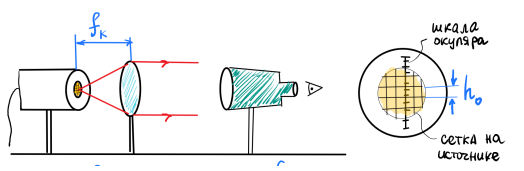
\includegraphics[width=8cm]{images/setup4(1).png}
        \caption{Схема установки для калибровки сетки}
    \end{subfigure}
    \hfill
    \begin{subfigure}{0.45\linewidth}
        \centering
        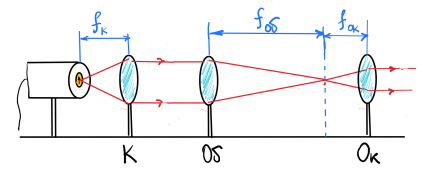
\includegraphics[width=8cm]{images/setup4(2).png}
        \caption{Схема телескопа Кеплера}
    \end{subfigure}
\end{figure}

\begin{figure}[h!]
    \centering
    \begin{subfigure}{0.45\linewidth}
        \centering
        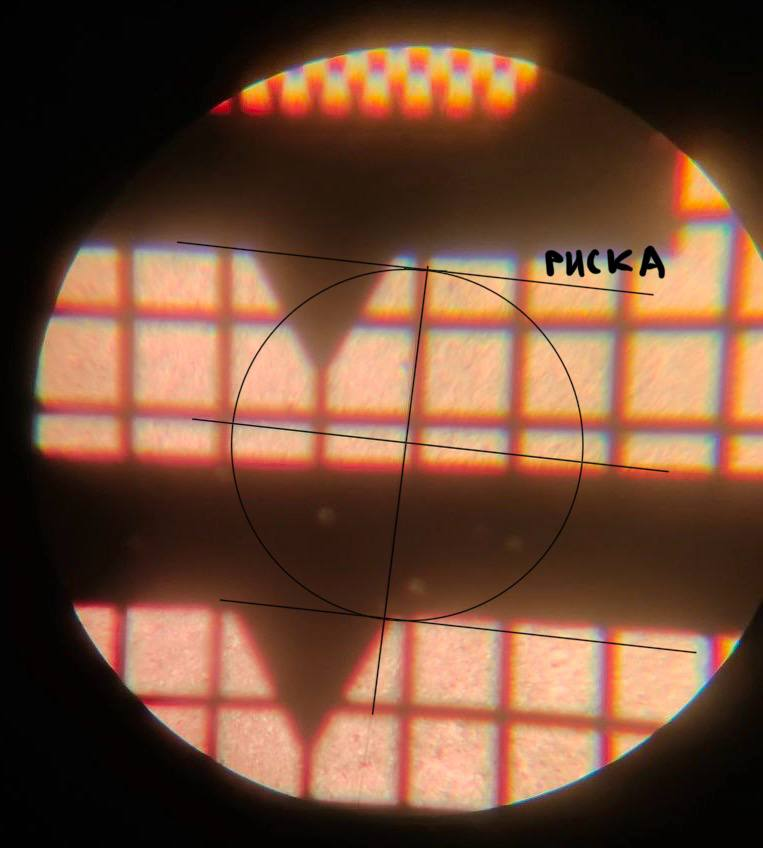
\includegraphics[width=9cm]{images/calibrate.jpg}
        \caption{Изображение сетки при калибровке}
    \end{subfigure}
    \hfill
    \begin{subfigure}{0.45\linewidth}
        \centering
        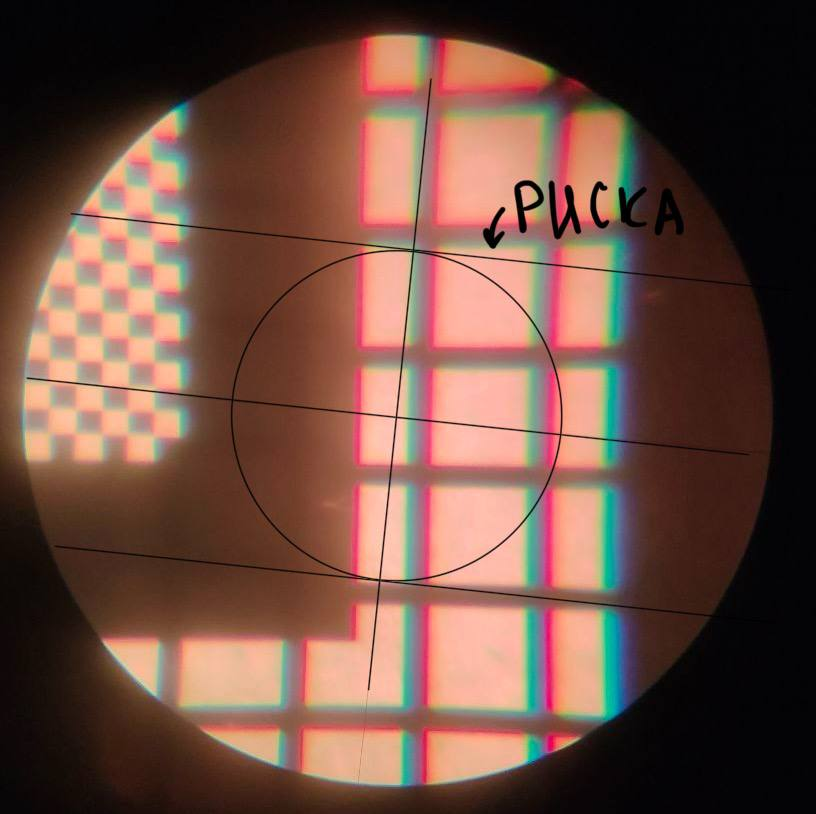
\includegraphics[width=9cm]{images/kepler_image.jpg}
        \caption{Увеличенное изображение в телескопе}
    \end{subfigure}
    \caption{Определение углового увеличения телескопа Кеплера}
\end{figure}


\subsection*{V. Сборка и изучение модели микроскопа}

\textit{Проекционный микроскоп}:
Изображение предмета в микроскопе можно сделать действительным и сфокусировать его на экране за окуляром (проекционный микроскоп). Увеличение проекционного микроскопа равно:

\begin{equation}
\gamma_{\text{пр}} = \frac{L - f_{\text{ок}}}{f_{\text{ок}}} \cdot \frac{\Delta}{f_{\text{об}}},
\end{equation}

где $L$ --- расстояние от окуляра до экрана.
\begin{figure}[h!]
    \centering
    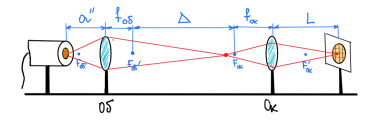
\includegraphics[width=14cm]{images/setup5.png}
    \caption {Схема микроскопа}
\end{figure}


\begin{figure}[h!]
    \centering
    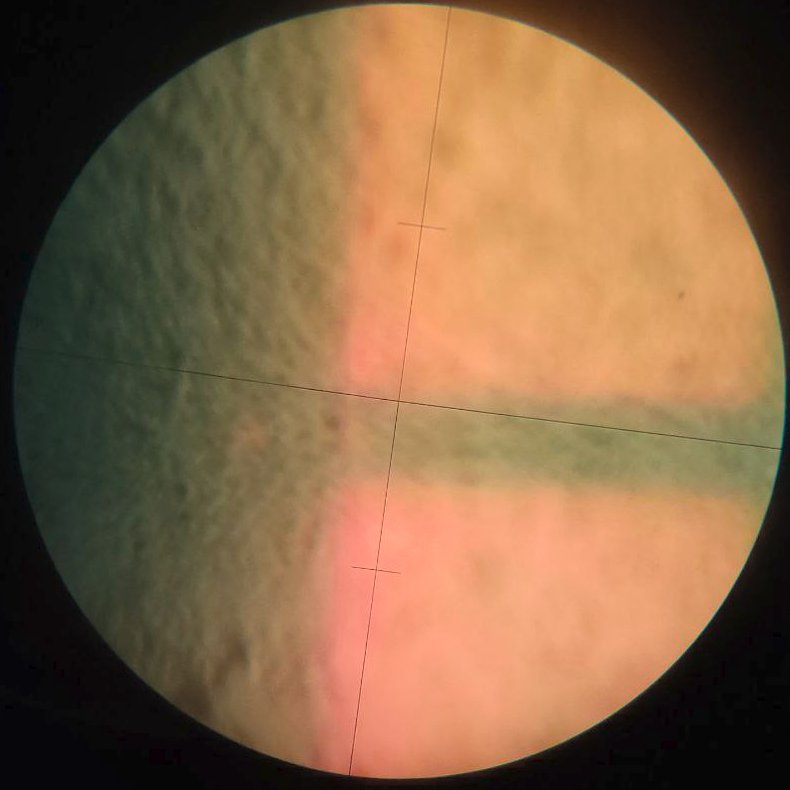
\includegraphics[width=9cm]{images/task5.jpg}
    \caption {Оценка увеличения "на глаз"}
\end{figure}

В качестве объектива и окуляра были выбраны линзы №4.6 $F_6 = 4.2$ см и №4.1 $F_1 = 4.1$ см cоответственно.\\
$$\bm{L = 29\textbf{ см}; \gamma = 5 \textbf{ см}};$$ \\$$\bm{\Delta x = \gamma \frac{f_{\textbf{об}} \cdot f_{\textbf{ок}}}{L - f_{\textbf{об}}} = 3.45 \textbf{ см}}$$

На глаз увеличение оценить сложно, но должно быть больше 5.
Отношение размера изображеия на экране к рамеру самого изображения $\alpha = \frac{4}{1.3} = 3.1$

\section*{Выводы}
\indent Были посчитаны фокусные расстояния линзы различными способами:\\
1) С помощью подзорной трубы $f_{4.2} = 10.1 \pm 0.2$ см\\
2) По формуле тонкой линзы $f_{4.2} = 12.4 \pm 0.2$ см\\
3) По формуле Бесселя $f_{4.2} = 12.5 \pm 0.03$ см\\
4) Методом Аббе $f_{4.2} = 9.1 \pm 0.1$ см\\

Вимдно, что значения колеблются около 10 см. По погрешности самым точным можно назвать метод Бесселя.
Так же для всех линз были определены фокусные расстояния (с помощью подзорной турбы) и с обратной стороны, чтобы можно было определить, можно ли считать линзу тонкой.
Разброс результатов не превышает 13\%, поэтому считаем линзы тонкими.\\
\indent Так же был собран телескоп Кеплера и определено его угловое увеличение: Экспериментально $\approx 1.5$ и теоретически $\approx 2.5$. Результат совсем не совпадают. Этом можно объяснить тем, что определять увеличение по изображеню на телескопе очень неточно и с учетом большой погрешности $\approx 50\%$ результат даже можно считать близким к теории.\\
\indent Был собран проекционный микрсокоп с увеличением 5. Что опять не сопадает с экспериментом - $\approx 3$\\




\end{document}
